% algorithms: 
% views: 
% containers: adjacency matrix
% data model: incoming edges on a vertex

\chapter{Introduction}
\label{ch:introduction}

\section{Motivation}

The original STL revolutionized the way that C++ programmers could apply algorithms to different kinds of containers, by defining \emph{generic} algorithms, realized via function templates.  
A hierarchy of \emph{iterators} were the mechanism by which algorithms could be made generic with respect to different kinds of containers,
Named requirements specified the valid expressions and associated types that algorithms required of their arguments.  As of C++20, we now have both ranges and concepts, which
now provide language-based mechanisms for specifying requirements for generic algorithms.

As powerful as the algorithms in the standard library are, the underlying basis for them is a range (or iterator pair), which inherently can only specify a one-dimensional container.  
Iterator pairs (equiv.\ ranges) specify a \lstinline{begin()} and an \lstinline{end()} and can move between those two limits in various ways, depending on the type of iterator.
As a result, important classes of problems that programmers are regularly faced with use structures that are not one-dimensional containers, and so the standard library algorithms can't be directly used.
Multi-dimensional arrays are an example of one such kind of data structure. Matrices do have the nice property that they (typically) have the ability to be ``raveled'', i.e., the data underlying the matrix can still be treated as a one-dimensional container.  Multi-dimensional arrays also have the property that, even though they can be thought of as hierarchical containers, the hierarchy is uniform---an N-dimensional array is a container of N-1 dimensional arrays.

Another important problem domain that does not fit into the category of one-dimensional ranges is that of \emph{graph algorithms and data structures}.
Graphs are a powerful abstraction for modeling relationships between entities in a given problem domain,
irrespective of what the actual entities are, and irrespective of what the actual relationships are.
In that sense, graphs are, by there very nature, generic.
Graphs are a fundamental abstraction in computer science, and are ubiquitous in real-world applications.

Any problem concerned with connectivity can be modeled as a graph.  
Just a small set of examples include
Internet routing, circuit partitioning and layout, finding the best route to take to a destination on map.
There are also relationships between entities that are inferred from large sets of data, for example the graph of consumers who have purchased the same product, or who have viewed the same movie.
Yet more interesting structures arise (hypergraphs or k-partite graphs) can arise when we want to model relationships between diverse types of data, such as the graph of consumers, the products they have purchased, and the vendors of the products.
And, of course, graphs play a critical role in multiple aspects of machine learning.

On the flip side of graph structures are the graph algorithms that are widely used for problems such as the above.
Well-known graph algorithms include breadth-first search, Dijkstra's algorithm, connected components, and so on.
%
Because graphs can come from so many different problem domains, they will also be represented with many different kinds of data structures.
To make graph algorithms as usable as possible across arbitrary representation requires application of the same principles that were used in the original STL: 
a collection of related algorithms from a problem domain (in our case, graphs),
minimizing the requirements imposed by the algorithms on their arguments,
systematically organizing the requirements, and
realizing this framework of requirements in the form of concepts.

There are also many uses of graphs that would not be met by a standard set of algorithms.  A standardized interface for graphs is eminently useful in such situations as well.  
In the most basic case, it would provide a well-defined framework for development.  But in keeping with the foundational goal of generic programming to enable reuse, it would also empower users to develop and deploy their own reusable graph components.  In the best case, such algorithms would be available to the broader C++ programmer community.

Because graphs are so ubiquitous and so important to modern software systems, a standardized library of graph algorithms and data structures would have enormous benefit to the C++ development community.
This proposal contains the specification of such a library, developed using the principles above.



\section{Example: Six Degrees of Kevin Bacon}
\label{sec:bacon}

A classic example of the use of a graph algorithm is the game ``The Six Degrees of Kevin Bacon.''
The game is played by connecting actors to each other through movies they have appeared in together.
The goal is to find the smallest number of movies that connect a given actor to Kevin Bacon.
That number is called the ``Bacon number'' of the actor. Kevin Bacon himself has a Bacon number of 0.
Since Kevin Bacon appeared with Tom Cruise in ``A Few Good Men'', Tom Cruise has a Bacon number of 1.

The following program computes the Bacon number for a small selection of actors.

% \phil{Duplicated in Overview's Examples}
{\small
  \lstinputlisting[firstline=26,lastline=49]{src/bacon.cpp}
}


\noindent
Output:
\begin{lstlisting}
Tom Cruise has Bacon number 1
Kevin Bacon has Bacon number 0
Hugo Weaving has Bacon number 3
Carrie-Anne Moss has Bacon number 4
Natalie Portman has Bacon number 2
Jack Nicholson has Bacon number 1
Kelly McGillis has Bacon number 2
Harrison Ford has Bacon number 1
Sebastian Stan has Bacon number 3
Mila Kunis has Bacon number 3
Michelle Pfeiffer has Bacon number 1
Keanu Reeves has Bacon number 4
Julia Roberts has Bacon number 1    
\end{lstlisting}  


In graph parlance, we are creating a graph where the vertices are actors and the edges are movies.
The number of movies that connect an actor to Kevin Bacon is the shortest path in the graph
from Kevin Bacon to that actor. In the example above, we compute shortest paths from Kevin
Bacon to all other actors and print the results.
Note, however, that actor-actor relationships are not how data about actors
is available in the wild (from IMDB, for example).  Rather, two types of  relationships available are actor-movie and movie-actor.  See Section~\ref{sec:multipartite} below.


\section{Graph Background} %  and Terminology}

For clarity, we briefly review some of the basic terminology of graphs.
We use commonly accepted terminology for graph data structures and algorithms and
adopt the particular terminology used in the textbook by
Cormen, Leiserson, Rivest, and Stein (``CLRS'')~\cite{CLRS2022}.

\subsection{Basic Terminology}

To model the relationships between entities, a \emph{graph} $G$ comprises two sets:
a \emph{vertex set} $V$, whose elements correspond to the entities, and an \emph{edge set} $E$, whose
elements are pairs corresponding to elements in $V$ that have some relationship with each other.  That is,
if $u$ and $v$ are members of $V$ that have some relationship that we wish to capture, then there is
a pair $\{u, v\}$ in $E$.  We can express that together $V$ and $E$ define a graph as $G=\{V, E\}$.

Two examples of graph models are shown in Figures~\ref{airport-summary} and~\ref{circuit-summary},
which respectively model a network of routes between and an electronic circuit.  
The figures show the domain-specific data to be modeled and the sets $V$ and $E$ for each graph.
Also shown for each graph is a
 node and link diagram, a commonly-used graphical\footnote{An unfortunate collision of terminology.}
notation.

\begin{figure}[ht]
  \begin{center}
    \subcaptionbox{An undirected graph representing airline routes between cities.  Shown are the list of airports (the vertices) and the list of routes between them (the  edges).  Also shown are a node and link diagram and the set-based description.\label{subfig:airport}}
    {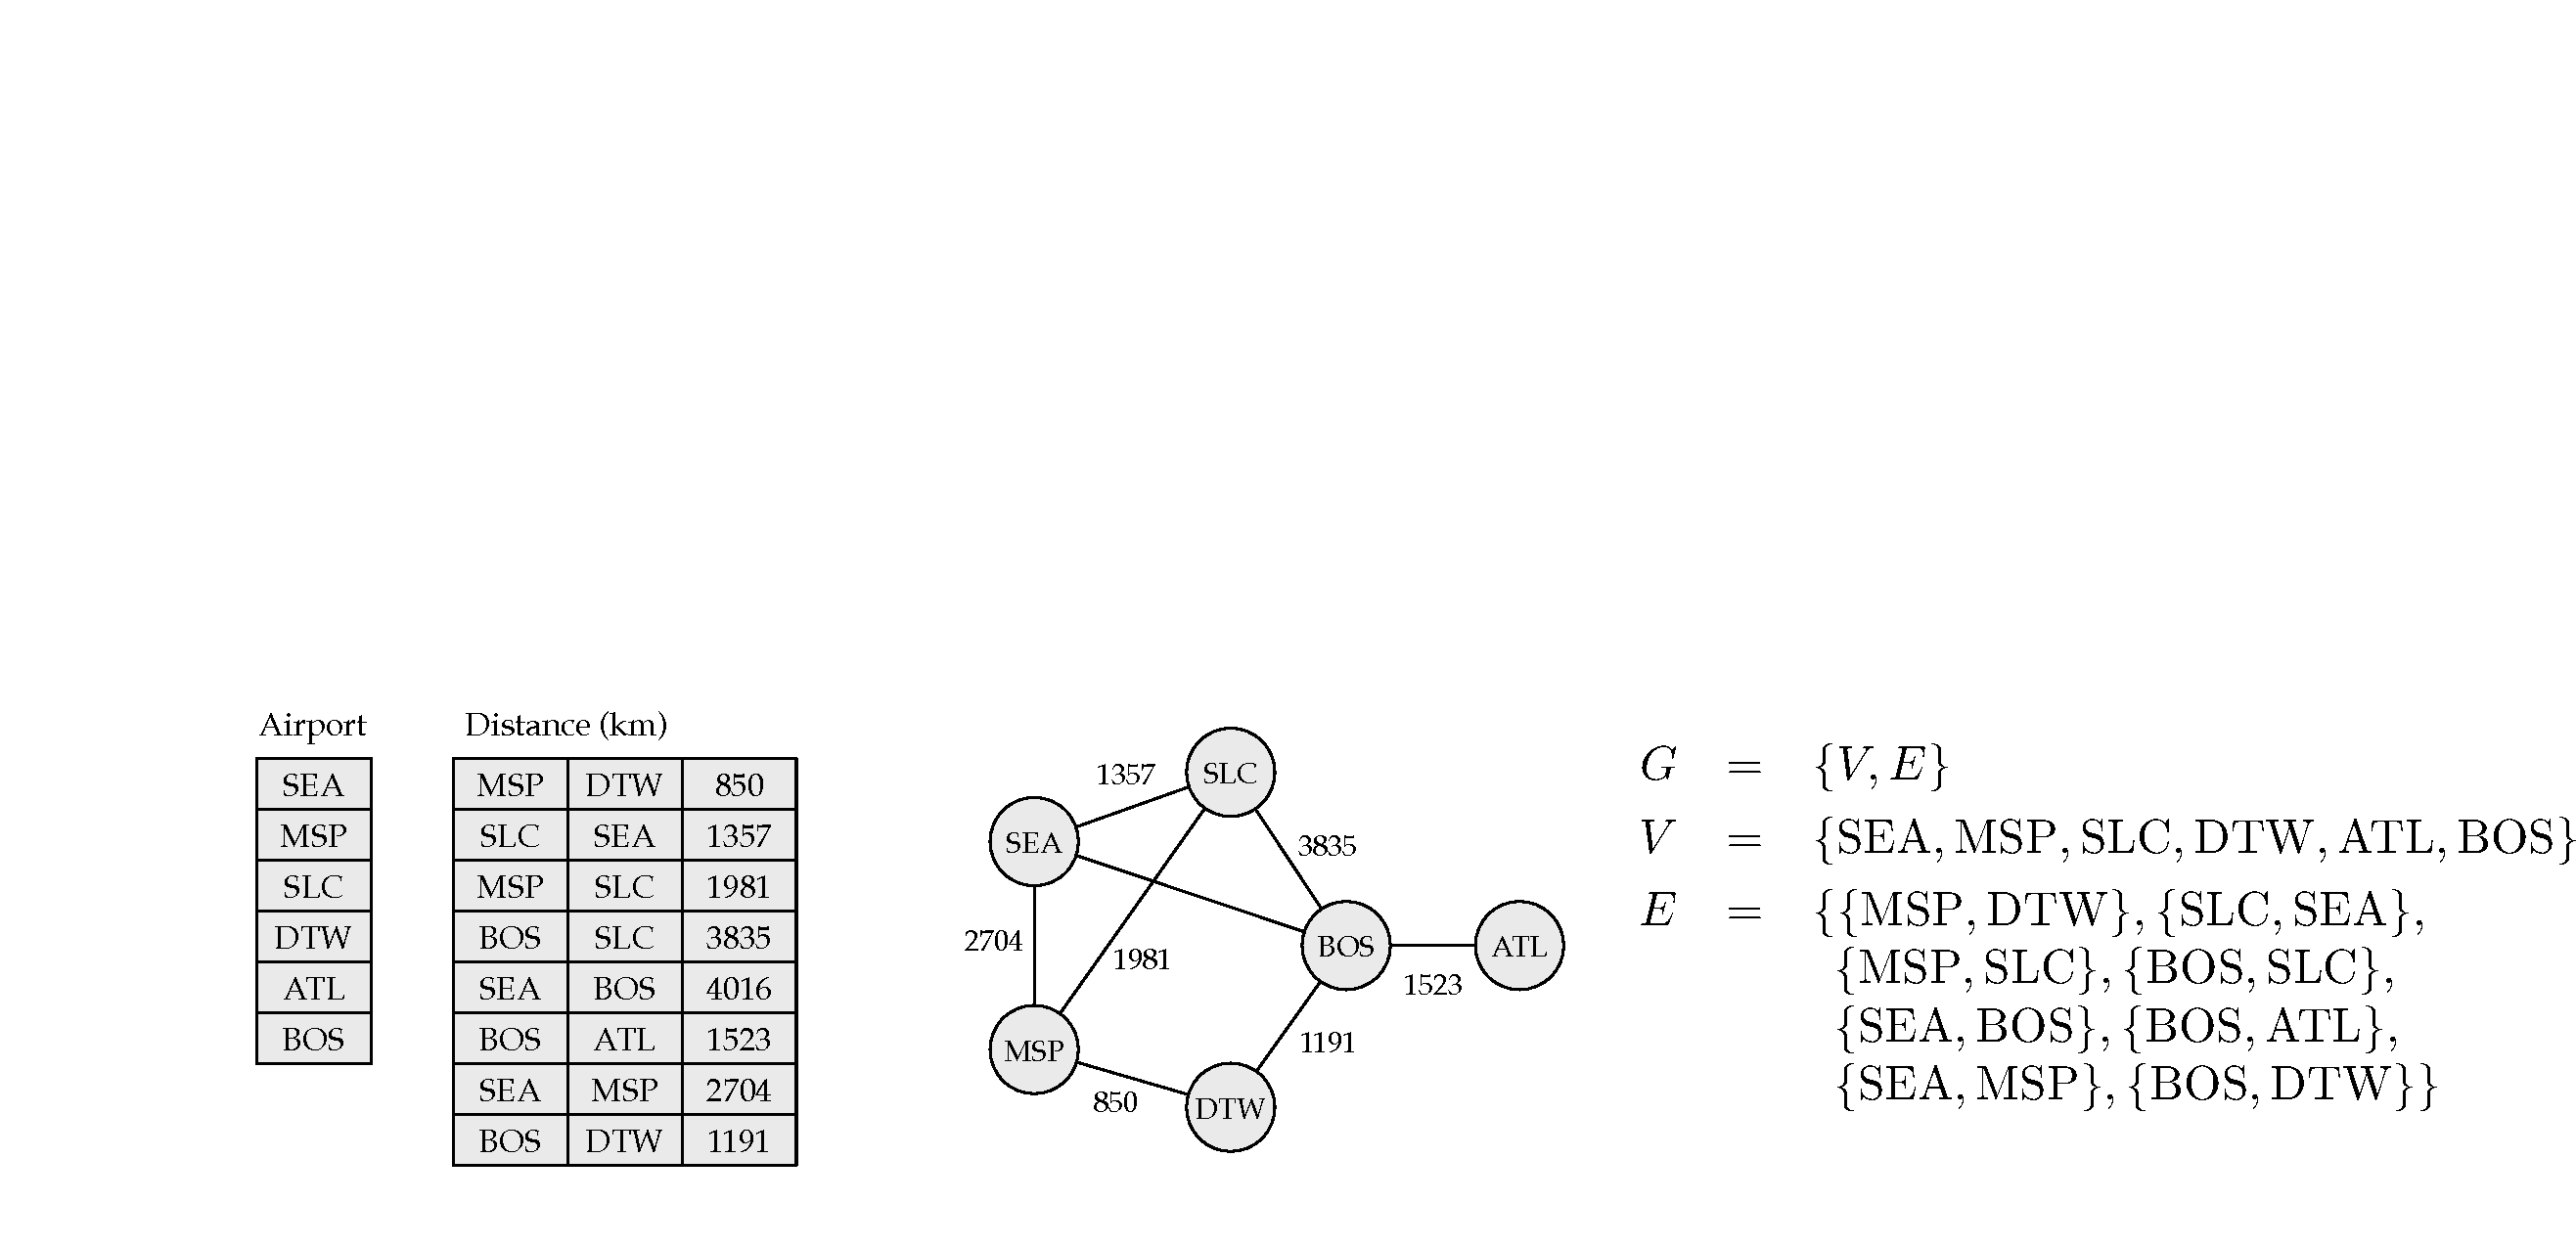
\includegraphics[width=0.75\textwidth]{figs/airport-summary.pdf}}
    \\
    \subcaptionbox{A directed graph representing an electronic circuit.  Shown in the circuit diagram are the labeled circuit nodes (the vertices) and the circuit elements connecting the nodes (the edges). Since circuit elements are oriented, we use a directed graph to model the circuit.  Also shown are a node and link diagram and the set-based decription.\label{subfig:circuit}}
    {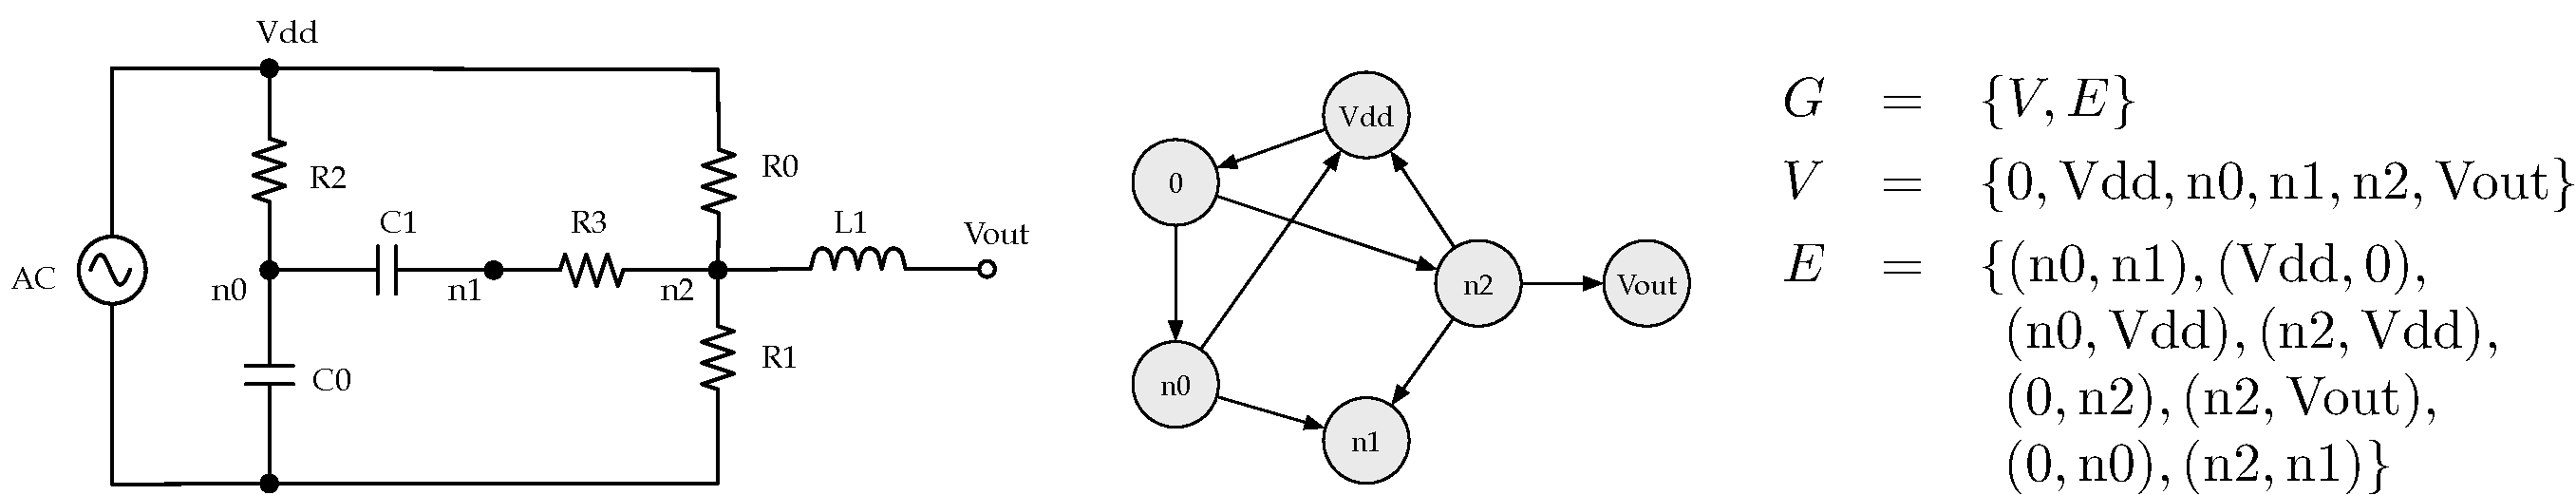
\includegraphics[width=0.825\textwidth]{figs/circuit-summary.pdf}}
    \caption{Graph models of an airline route system and of an electronic circuit.\label{fig:node_link_graphs}}
  \end{center}
\end{figure}


\subsection{Graph Representation: Enumerating the Vertices}

To reason about graphs, and to write algorithms for them, we require a \emph{representation} of the graph.
We note that \emph{a graph and its representation are not the same thing}.  It is therefore essential
that we be precise about this distinction as we develop a software library of graph
algorithms and data structures\footnote{In fact, if we are to be completely precise, the library we are
proposing is one of algorithms and data structures for graph representations.  We will make concessions
to commonly accepted terminology, while precisely defining that terminology.}.

The representations that we will be using are familiar ones: adjacency matrix, edge list, and adjacency list.
We begin with a process that is so standard that we typically don't even notice it, but it forms
the foundation of graph representations: we \emph{enumerate the vertices.}  That is, we assign an
index to each element of $V$ and write $V = \{v_0, v_1, \ldots v_{n-1}\}$.  Based on that enumeration,
elements of $E$ are expressed in the form $\{v_i, v_j\}$.  Similarly, we can enumerate the edges, and write  
$E = \{ e_0, e_1, \ldots e_{m-1}\}$, though the enumeration of $E$ does not play a role in standard
representations of graphs.
%
The number of elements in $V$ is denoted by $|V|$ and the number of elements in $E$ is denoted by $|E|$.

We summarize some remaining terminology about vertices and edges.
\begin{itemize}
\item 
An edge $e_k$ may  be \emph{directed}, denoted as the ordered pair $e_k=(v_i, v_j)$, or it may be
  \emph{undirected}, denoted as the (unordered) set $e_k=\{v_i, v_j\}$.  The edges 
in $E$ are either all directed or all undirected,
  corresponding respectively to a \emph{directed graph} or to an \emph{undirected} graph.
\item 
If the edge set $E$ of a directed graph contains an edge $e_k = (v_i,v_j)$, then
  vertex $v_j$ is said to be \emph{adjacent} to vertex $v_i$.  The edge $e_k$ is an
  \emph{out-edge} of vertex $v_i$ and an in-edge of vertex $v_j$.  Vertex $v_i$ is the \emph{source} of
  edge $e_k$, while $v_j$ is the \emph{target} of edge $e_k$.
\item If the edge set $E$ of an undirected graph contains an edge $e_k = \{v_i,v_j\}$, then
  $e_k$ is said to be \emph{incident} on the vertices $v_i$ and $v_j$.
  Moreover, vertex $v_j$ is adjacent to vertex $v_i$
  \emph{and} vertex $v_i$ is adjacent to vertex $v_j$.
  The edge $e_k$ is an out-edge of both $v_i$ and $v_j$ and it is an in-edge of both $v_i$ and $v_j$.
\item The \emph{neighbors} of a vertex $v_i$ are all the vertices $v_j$ that are adjacent to $v_i$.  The set of all of the neighbors is the \emph{neighborhood} of $v_i$.
\item A \emph{path} as a sequence of vertices $v_0, v_1, \ldots, v_{k-1}$ such that
there is an edge from $v_0$ to $v_1$, an edge from $v_1$ to $v_2$, and so on.
That is, a path is a set of edges $(v_i, v_{i+1}) \in E$ for  $i = 0, 1, \ldots, k-2$.
\end{itemize}


\subsection{Adjacency-Based Representations}

We begin our development of graph representations
with the almost universally-accepted definition of the
adjacency matrix representation of a graph.
%
The \emph{adjacency matrix representation} of a graph $G$ is a $|V|\times |V|$ matrix $A = (a_{ij})$ such that,
respectively for a directed or undirected graph
\[
 a_{i j} = 
 \left\{
 \begin{array}{rl}
  1 & \textrm{if } (v_i, v_j) \in E \\
  0 & \textrm { otherwise }
 \end{array}
 \right.
 \qquad\qquad
 a_{i j} = a_{ji} =
 \left\{
 \begin{array}{rl}
  1 & \textrm{if } (v_i, v_j) \in E \\ 
  0 & \textrm { otherwise }
 \end{array}
 \right.
\]
That is, $a_{ij} = 1$ if and only if $v_j$ is adjacent to $v_i$ in the original graph $G$ (hence the name ``adjacency matrix``).
%
Here we can see why we said that the initial enumeration of $V$ is foundational to representations:  \emph{The adjacency matrix is based solely on the indices used in that enumeration}.  It does not contain the vertices or edges themselves.

As a data structure to use for algorithms, the adjacency matrix is not very efficient, neither in terms of storage (which, at $|V|\times |V|$ is prohibitive), nor for computation. Instead of storing the entire
adjacency matrix, we can simply store the index values of its non-zero elements.  A \emph{sparse coordinate adjacency
matrix} is a container $C$ of pairs $(i, j)$ for every $a_{ij}$ in $A$.
%
At first glance, it may seem that we have simply created a data structure $C$ that has a pair $(i,j)$ if $E$ in the
original graph has an edge from $v_i$ to $v_j$.  This is true in the directed case.  However, in the undirected case, if there is an edge between $v_i$ and $v_j$, then $v_i$ is adjacent to $v_j$ and $v_j$ is adjacent to $v_i$.  In other words, if there is an edge between $v_i$ and  $v_j$ in an undirected graph, then both the entries $a_{ij}$ and $a_{ji}$ are equal to $1$\footnote{That is, the adjacency matrix is symmetric.} --- and therefore for a single edge between $v_i$ and $v_j$,  $C$ contains two index pairs: $(i, j)$  and $(j, i)$.   The sparse coordinate representation is commonly known as \emph{edge list}.  However, we caution the reader that $C$ does not store edges, but rather indices and that, in the case that it represents an undirected graph, there is not a 1-1 correspondence between the edges in $E$ and the contents of $C$.

Although the sparse coordinate adjacency matrix is much more efficient in terms of storage than the original adjacency matrix, it isn't as efficient as it could be.  
Much more importantly, it does not at all useful for the types of operations used by most graph algorithms, which need to be able to get the set of neighbors of a given vertex in constant time.  
To support this type of operation, we use a \emph{compressed sparse adjacency matrix}, which is an array $J$ with $|V|$ entries, where each $J[i]$ is a linear container of indices $\{ j \}$ such that $v_j$ is a neighbor of $v_i$ in $G$.  
That is $j$ is contained in $J[i]$ if and only if there is an edge $(v_i, v_j)$ in $E$ (or, equivalently, if there is a pair $(i, j)$ in $C$ or, equivalently, if $a_{ij} = 1$)\footnote{The compressed sparse adjacency matrix is identical to the compressed sparse row format from linear algebra}.  
We note that if $(v_i, v_j)$ is an edge in an undirected graph, $J[i]$ will contain $j$ and $J[j]$ will contain $i$. 
The common name for this data structure is \emph{adjacency list}.  
Although this name is problematic (for instance, it is not actually a list),  it is so widely used that we also use it here---but \emph{we mean specifically that an  ``adjacency list'' is the compressed sparse adjacency matrix representation of a graph}\footnote{We concede that ``adjacency list'' rolls off the tongue much more easily than ``compressed sparse adjacency matrix representation of a graph.''}.  
Again we emphasize the distinction between a graph and its representation:  An adjacency list $J$ is not the same as the graph $G$---it is a representation of $G$.


Illustrations of the adjacency-matrix representations of the airline route graph and the electronic circuit graph are shown in Figures~\ref{fig:airport} and~\ref{fig:circuit}, respectively.

\begin{figure}[bh]
  \begin{subfigure}[t]{0.175\textwidth}
    \centering
    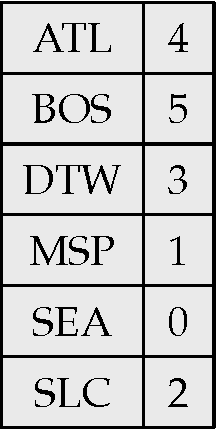
\includegraphics[width=0.4\linewidth]{airport-vertex-enumeration}
    \caption{\label{fig:ariport-vertex-enumeration}
    An enumeration of the airport graph given in \protect\ref{subfig:airport}.}
  \end{subfigure}
  \hspace{1em}
  \begin{subfigure}[t]{0.25\textwidth}
    \centering
    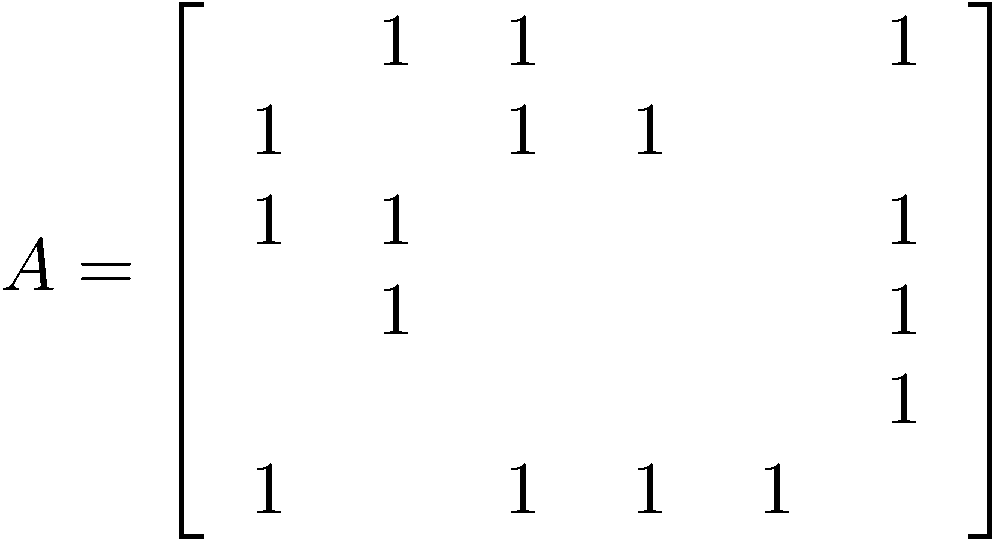
\includegraphics[width=\linewidth]{airport-graph-adjacency-matrix}
    \caption{\label{fig:airport-graph-adjacency-matrix}
    The adjacency matrix representation of the graph given in Figure~\protect\ref{subfig:airport},
    using the enumeration given in Figure~\protect\ref{fig:airport-vertex-enumeration}.}
  \end{subfigure}
  \hspace{1em}
  \begin{subfigure}[t]{0.175\textwidth}
    \small
    \centering
    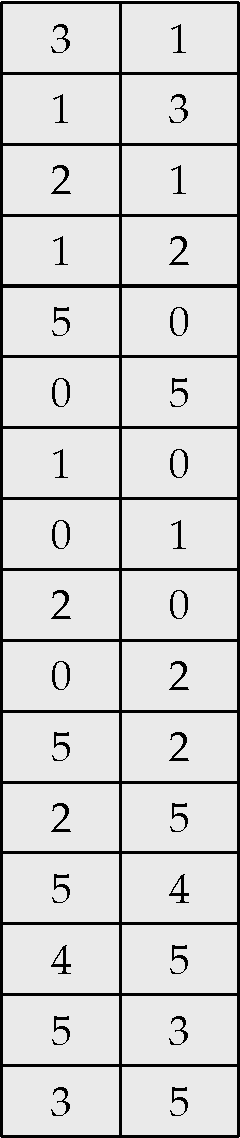
\includegraphics[width=0.4\linewidth]{airport-coordinate-sparse-adjacency}
    \caption{\label{fig:airport-coordinate-sparse-adjacency}
    The coordinate sparse adjacency matrix representation.}
  \end{subfigure}
  \hspace{1em}
  \begin{subfigure}[t]{0.3\textwidth}
    \small
    \centering
    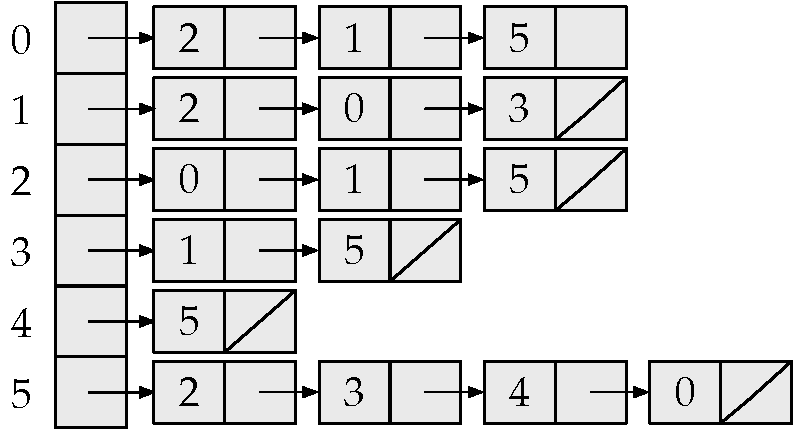
\includegraphics[width=0.75\linewidth]{airport-compressed-sparse-adjacency}
    \caption{\label{fig:airport-compressed-sparse-adjacency}
    The compressed sparse adjacency matrix representation.}
  \end{subfigure}
  \caption{Adjacency matrix representations of the airport graph model.\label{fig:airport-representation}}
\end{figure}



\begin{figure}[bh]
  \begin{subfigure}[t]{0.175\textwidth}
    \centering
    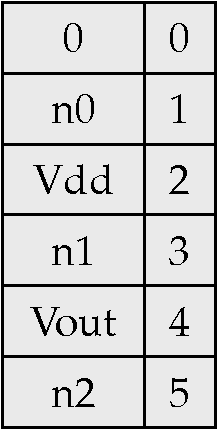
\includegraphics[width=0.4\linewidth]{circuit-vertex-enumeration}
    \caption{\label{fig:circuit-vertex-enumeration}
    An enumeration of the circuit graph given in \protect\ref{subfig:circuit}.}
  \end{subfigure}
  \hspace{1em}
  \begin{subfigure}[t]{0.25\textwidth}
    \centering
    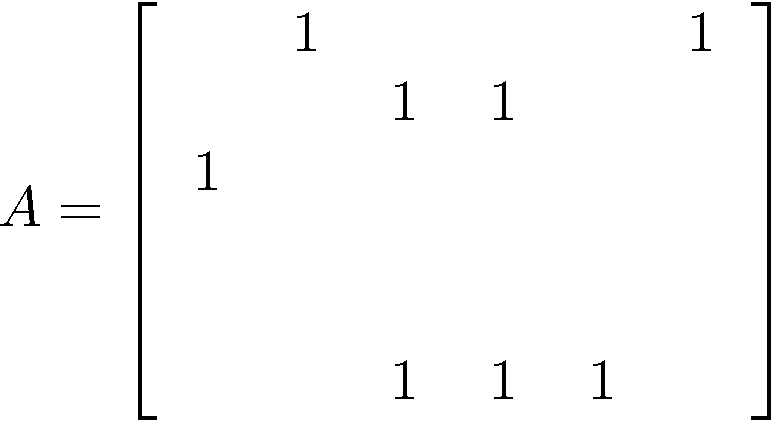
\includegraphics[width=\linewidth]{circuit-graph-adjacency-matrix}
    \caption{\label{fig:circuit-graph-adjacency-matrix}
    The adjacency matrix representation of the graph given in Figure~\protect\ref{subfig:circuit},
    using the enumeration given in Figure~\protect\ref{fig:circuit-vertex-enumeration}.}
  \end{subfigure}
  \hspace{1em}
  \begin{subfigure}[t]{0.175\textwidth}
    \small
    \centering
    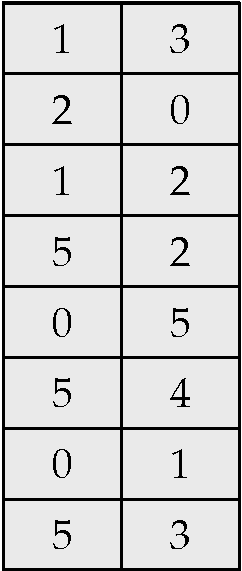
\includegraphics[width=0.4\linewidth]{circuit-coordinate-sparse-adjacency}
    \caption{\label{fig:circuit-coordinate-sparse-adjacency}
    The coordinate sparse adjacency matrix representation.}
  \end{subfigure}
  \hspace{1em}
  \begin{subfigure}[t]{0.3\textwidth}
    \small
    \centering
    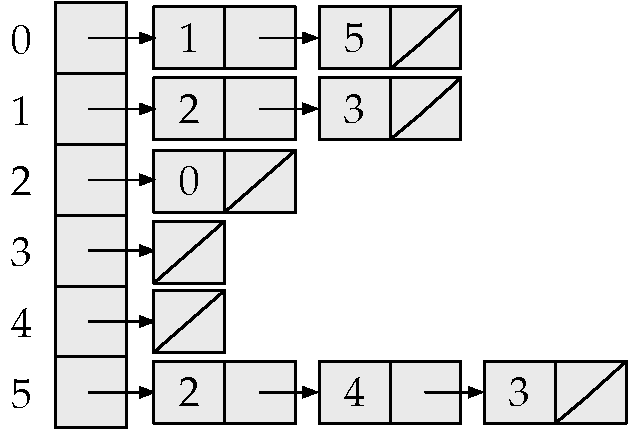
\includegraphics[width=0.75\linewidth]{circuit-compressed-sparse-adjacency}
    \caption{\label{fig:circuit-compressed-sparse-adjacency}
    The compressed sparse adjacency matrix representation.}
  \end{subfigure}
  \caption{Adjacency matrix representations of the circuit graph model.\label{fig:circuit-model}}
\end{figure}


\subsection{From Data to Graph}


Consider again the circuit diagram shown in Figure~\ref{subfig:circuit}.  We  model the circuit as a graph, identifying  nodes in the circuit as vertices, and circuit elements in the circuit as directed edges (since circuit elements are oriented).
 Since circuit elements are oriented, we identify them with directed edges.  Thus, the graph model for the
circuit is directed.  
\[
\begin{array}{rcl}
  G & = & \{ V, E \} \\[\smallskipamount]
        V & = & \{ \mathrm{0}, \mathrm{Vdd}, \mathrm{n0}, \mathrm{n1}, \mathrm{n2}, \mathrm{Vout} \} \\[\smallskipamount]
        E & = & \{
        ( \mathrm{n0}, \mathrm{n1} ),  ( \mathrm{Vdd}, \mathrm{0} ),
        ( \mathrm{n0}, \mathrm{Vdd} ), ( \mathrm{n2}, \mathrm{Vdd} )\\
        &&\:\:
        ( \mathrm{0}, \mathrm{n2} ),  ( \mathrm{n2}, \mathrm{Vout} ),
        ( \mathrm{0}, \mathrm{n0} ),  ( \mathrm{n2}, \mathrm{n1} ) \}
      \end{array}
\]


A diagram of the graph model for the circuit is shown in Figure~\ref{fig:circuit-graph-no-edge-labels} and the mathematical representation for the graph is shown
  in Figure~\ref{fig:circuit-graph-math}.
  \item We enumerate the vertices of the graph given in Figure~\ref{fig:circuit-graph-math} from $0$ to $5$, as
  shown in Figure~\ref{fig:circuit-vertex-enumeration}.  Using this enumeration, we can construct an adjacency matrix,
  as shown in

\begin{figure}[bh]
  \begin{subfigure}[t]{0.175\textwidth}
    \centering
    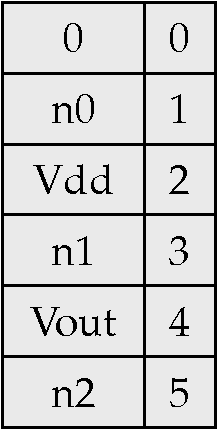
\includegraphics[width=0.4\linewidth]{circuit-vertex-enumeration}
    \caption{\label{fig:circuit-vertex-enumeration}
    An enumeration of the circuit graph given in \protect\ref{subfig:circuit}.}
  \end{subfigure}
  \hspace{1em}
  \begin{subfigure}[t]{0.25\textwidth}
    \centering
    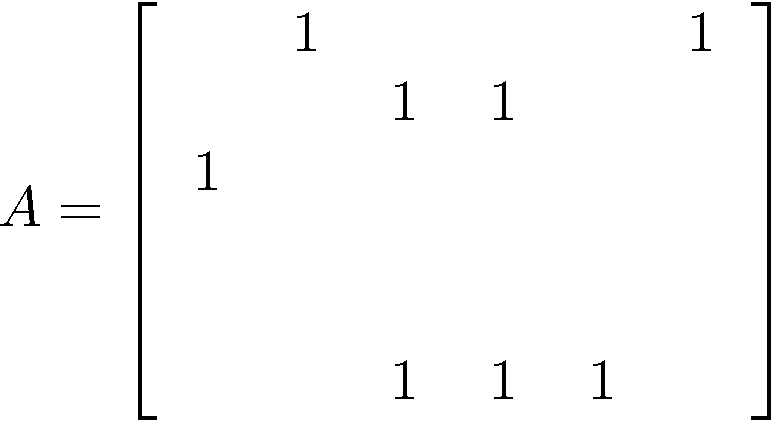
\includegraphics[width=\linewidth]{circuit-graph-adjacency-matrix}
    \caption{\label{fig:circuit-graph-adjacency-matrix}
    The adjacency matrix representation of the graph given in Figure~\protect\ref{subfig:circuit},
    using the enumeration given in Figure~\protect\ref{fig:circuit-vertex-enumeration}.}
  \end{subfigure}
  \hspace{1em}
  \begin{subfigure}[t]{0.175\textwidth}
    \small
    \centering
    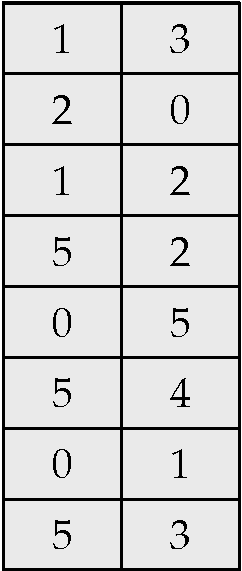
\includegraphics[width=0.4\linewidth]{circuit-coordinate-sparse-adjacency}
    \caption{\label{fig:circuit-coordinate-sparse-adjacency}
    The coordinate sparse adjacency matrix representation.}
  \end{subfigure}
  \hspace{1em}
  \begin{subfigure}[t]{0.3\textwidth}
    \small
    \centering
    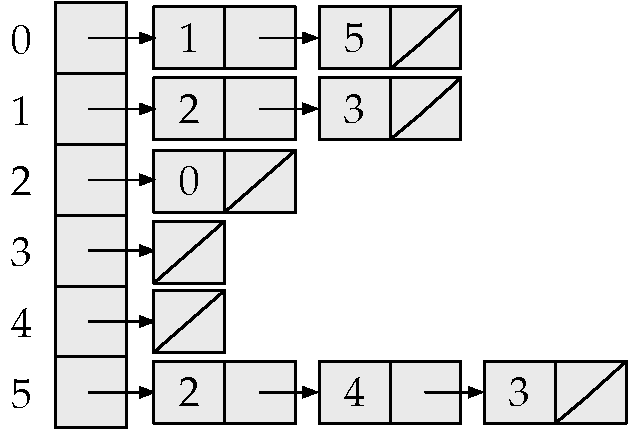
\includegraphics[width=0.75\linewidth]{circuit-compressed-sparse-adjacency}
    \caption{\label{fig:circuit-compressed-sparse-adjacency}
    The compressed sparse adjacency matrix representation.}
  \end{subfigure}
  \caption{Adjacency matrix representations of the circuit graph model.}
\end{figure}





\section{MultiPartite Graphs}
\label{sec:multipartite}

\andrew{
Need some definitions to properly include -- or exclude -- general labeled graphs.
}

\phil{Need to reword to accomodate multipartite graphs}
So far, we have been considering graphs where the vertices are in a single set $V$
and the edges are pairs of elements from $V$.  
%
% We refer to such a graph as a \emph{unipartite} graph.
%
But consider again the Kevin Bacon example.  The source for the information comprising the
Kevin Bacon data is the Internet Movie Database (IMDB).  However, the IMDB does not contain
the relationships between actors.  Rather it contains files of tabular data, one of which
contains an entry for each movie with the list of actors that have appeared in that movie,
and one of which contains an entry for each actor with the list of movies that actor has
appeared in (``movie-actor'' and ``actor-movie'' tables, respectively).

A graph, as we have previously defined it, cannot model the IMDB.  The relationships
contained in the data are between actors and movies.



, and both elements of an
edge, are members of a single set $|V|$. A graph with a single vertex set is called a
\emph{unipartite} graph. If the vertices in a graph can be partitioned into two
disjoint sets such that all of the edges in the graph only connect vertices from one
set of the vertices of the other set, the graph is called a \emph{bipartite} graph.
\andrew{Set membership == vertex label.  How many labels can a vertex have?  How many sets can a vertex belong to?}

Even if a graph is designated to be unipartite, it may be the case that its vertices
can be partitioned into two disjont sets. In such a case, the graph is bipartite,
but as a run-time property, not a compile-time property.
That is, determining whether a given graph is bipartite requires a run-time analysis
of the graph, with an appropriate algorithm.

However, there are numerous cases of interest where the vertices of a graph fall
naturally into two disjoint sets. For example, in the
in a social network, the vertices
represent people and the edges represent friendships. In such a case, it is natural
Of particular interest for realizing a bipartite graph is when the graph is
structurally bipartite, that is, when we are explicitly given two different
sets of vertices and the corresponding set of edges that connect vertices of the two sets.
This common---and important---use case arises when modeling relationships
between different types of entities. For example, we might use a structurally
bipartite graph in which one vertex set represents customers and another vertex
set represents products. An edge between a customer and a product would be used
to indicate that a customer has purchased a particular product.
Another such example is from the Kevin Bacon game above, where
one set represents actors and the other set represents movies; edges represent whether
and actor appeared in a movie. Thus edges only connect vertices from the set of actors
to the set of movies.

We can refer to graphs of this form as \emph{structurally bipartite} graphs and
denote them as $G = (U, V, E)$, where the vertex sets $U$ and $V$ are disjoint.

\subsection{BiPartite Graph Models}

\subsection{BiPartite Graph Implementations}



\section{From Data to Graph}

\subsection{Columnar Data}

Figure~\ref{fig:edge_list_from_columnar_data}
shows how one might create an unlabeled edge list from a table of data stored in a CSV file.
The values in each row are assumed to be separated by whitespace.
The elements of the first column are considered to be the source vertices and the elements of
the second column are the destination vertices. For edges with properties, the third column
contains the property values.

\begin{figure}[ht]
  \begin{center}
    \begin{subfigure}{0.48\textwidth}
      \begin{lstlisting}[language=C++]
    auto directed_edge_list<vertex_id_t, vertex_id_t>
      std::vector<std::tuple<vertex_id_t, vertex_id_t> edges;
    auto input = std::ifstream ("input.csv");
    vertex_id_t src, dst;
    while (input >> src >> dst) {
        edges.emplace_back (src, dst);
    }
      \end{lstlisting}
      \caption{Creating a directed edge list with no edge properties.
      The edge list container is a vector of tuples.
      \label{subfig:edge_list_no_properties}}
    \end{subfigure}
    \begin{subfigure}{0.48\textwidth}
      \begin{lstlisting}[language=C++]
    auto undirected_edge_list_graph<vertex_id_t, vertex_id_t, double>
      graph<std::vector<vertex_id_t>, std::vector<vertex_id_t>, std::vector<double>> edges;
    auto input = std::ifstream ("input.csv");
    vertex_id_t src, dst;
    double val;
    while (input >> src >> dst >> val) {
        edges.emplace_back (src, dst, val);
    }
      \end{lstlisting}
      \caption{Creating an undirected edge list with edge properties.
      The edge list container is comprised of three vectors, wrapped by
      the `lstinline{graph}' adapter.
      \label{subfig:edge_list_with_properties}}
    \end{subfigure}
    \caption{Creating an edge list from columnar data.\label{fig:edge_list_from_columnar_data}}
  \end{center}
\end{figure}

These examples are meant to be illustrative and not necessarily
comprehensive (nor efficient).
There are, of course, many ways to define containers that meet the
requirements of the edge list concept and many ways to
create an edge list from columnar data.

\subsection{Converting an Edge List to an Adjacency List}

\begin{figure}[ht]
  \begin{center}
    \begin{subfigure}{0.48\textwidth}
      \begin{lstlisting}[language=C++]
    auto edge_list<vertex_id_t, vertex_id_t> std::vector<std::tuple<vertex_id_t, vertex_id_t> edges;
    auto adjacency_list<vertex_id_t> std::vector<std::vector<vertex_d_t>> adj_list;
    for (auto [src, dst] : edges) {
      if (src >= adj_list.size()) {
        adj_list.resize(src + 1);
      }
      adj_list[src].push_back (dst);
    }
      \end{lstlisting}
      \caption{Creating an adjacency list from a directed edge list.
      The adjacency list container is a vector of vectors.
      \label{subfig:adj_list_from_directed_edge_list}}
    \end{subfigure}
    \begin{subfigure}{0.48\textwidth}
      \begin{lstlisting}[language=C++]
    auto edge_list_graph<vertex_id_t, vertex_id_t>
      graph<std::vector<std::tuple<vertex_id_t, vertex_id_t>> edges;
    auto adjaceny_list_graph<vertex_id_t, vertex_id_t, double>
      graph<std::vector<std::vector<vertex_d_t>, std::vector<double>> adj_list{edges.num_vertices()};
    for (auto [src, dst, val] : edges) {
      adj_list[src].push_back (dst, val);
      adj_list[dst].push_back (src, val);
    }
      \end{lstlisting}
      \caption{Creating an adjacency list from an undirected edge list with properties.
      Since the edges in the edge list are undirected, for a given edge $(u, v, w)$,
        $u$ is a neighbor of $v$ and $v$ is a neighbor of $u$. Thus, we insert both
        $(u, v, w)$ and $(v, u, w)$ into the adjacency list.
        The adjacency list container is comprised of three vectors, wrapped by
        the `lstinline{graph}' adapter.
        \label{subfig:adj_list_from_undirected_edge_list}}
    \end{subfigure}
    \caption{Creating an adjacency list from an edge list with properties.\label{fig:adj_list_from_edge_list}}
  \end{center}
\end{figure}

\andrew{We should have note that anything wrapped in a graph adapter has a `num\_vertices`
method (and other members).
We should also provide a constructor for the adapted adjacency list that takes and
edge list as argument.}


% The examples above basically cover what I intened here.  Though perhaps we should
% explain in some more detail about what the concepts do, what kinds of things meet
% concept requirements, what the graph adapter does, etc.
% \section{Implementations}
% But maybe we can just cover those things further down and forward reference to
% them from here.

% \subsection{Edge List: Array of Structs / Struct of Arrays}
% \andrew{Edges can be stored as tuples (or tuple like) basically in parallel arrays (like a ranges::zip).}
% \subsection{Vertices and Edges: Node Objects and Link Objects}
% \andrew{ala Stanford Graph Base (et al).}
% \subsection{Adjacency List: Container of Containers}
% \andrew{An adjacency list can be represented as a container of containers (e.g., std::vector<std::list>).  Talk about range of ranges when we talk about library interfaces, requirements, concepts.  Note here that the structure of an adjacency list does not capture directedness -- directedness is a run-time property.}


% These are definitely already covered in the examples above.
% \subsection{From Edge List to Adjacency List}
% \andrew{Scan edge list and insert edgest into adjacency list.  Adjacency list must support insertion.}
% \subsection{Edge List and Adjacency List: Compressed Edge List}
% \andrew{Using a sort and group-by (or a sort, a run-length encoding, and a scan), we can compactify the edge-list reprentation and at the same time obtain an adjacency-list representation -- one that is memory and compute efficient.  Best of both worlds.  Has same basic structural principles as CSR / CSC matrices in linear algebra -- but much more general.}



\section{Naming Conventions}


Table~\ref{tab:name_conv} shows the naming conventions used throughout this document.

\begin{table}[h!]
  \begin{center}
  {\begin{tabular}{l l l p{7cm}}
     \hline
     \textbf{Template}  &                                   & \textbf{Variable}    &                                                                                                                                                                                                  \\
     \textbf{Parameter} & \textbf{Type Alias}               & \textbf{Names}       & \textbf{Description}                                                                                                                                                                             \\
     \hline
     \tcode{G}          &                                   &                      & Graph                                                                                                                                                                                            \\
     & \tcode{graph_reference_t<G>}      & \tcode{g}            & Graph reference                                                                                                                                                                                  \\
     \tcode{GV}         &                                   & \tcode{val}          & Graph Value, value or reference                                                                                                                                                                  \\
     \hline
     \tcode{V}          & \tcode{vertex_t<G>}               &                      & Vertex                                                                                                                                                                                           \\
     & \tcode{vertex_reference_t<G>}     & \tcode{u,v,x,y}      & Vertex reference. \tcode{u} is the source (or only) vertex. \tcode{v} is the target vertex.                                                                                                      \\
     \tcode{VId}        & \tcode{vertex_id_t<G>}            & \tcode{uid,vid,seed} & Vertex id. \tcode{uid} is the source (or only) vertex id. \tcode{vid} is the target vertex id.                                                                                                   \\
     \tcode{VV}         & \tcode{vertex_value_t<G>}         & \tcode{val}          & Vertex Value, value or reference. This can be either the user-defined value on a vertex, or a value returned by a function object (e.g. \tcode{VVF}) that is related to the vertex.              \\
     \tcode{VR}         & \tcode{vertex_range_t<G>}         & \tcode{ur,vr}        & Vertex Range                                                                                                                                                                                     \\
     \tcode{VI}         & \tcode{vertex_iterator_t<G>}      & \tcode{ui,vi}        & Vertex Iterator. \tcode{ui} is the source (or only) vertex.                                                                                                                                      \\
     &                                   & \tcode{first,last}   & \tcode{vi} is the target vertex.                                                                                                                                                                                    \\
     \tcode{VVF}        &                                   & \tcode{vvf}          & Vertex Value Function: vvf(u) $\rightarrow$ vertex value                                                                                                                                         \\
     \tcode{VProj}      &                                   & \tcode{vproj}        & Vertex descriptor projection function: \tcode{vproj(x)} $\rightarrow$ \tcode{vertex_descriptor<VId,VV>}.                                                                                         \\
     \hdashline
                        & \tcode{partition_id_t<G>}         & \tcode{pid}          & Partition id.                                                                                                                                                                                    \\
                        &                                   & \tcode{P}            & Number of partitions.                                                                                                                                                                            \\
     \tcode{PVR}        & \tcode{partition_vertex_range_t<G>} & \tcode{pur,pvr}    & Partition vertex range.                                                                                                                                                                          \\
     \hline
     \tcode{E}          & \tcode{edge_t<G>}                 &                      & Edge                                                                                                                                                                                             \\
     & \tcode{edge_reference_t<G>}       & \tcode{uv,vw}        & Edge reference. \tcode{uv} is an edge from vertices \tcode{u} to \tcode{v}. \tcode{vw} is an edge from vertices \tcode{v} to \tcode{w}.                                                          \\
     \tcode{EV}         & \tcode{edge_value_t<G>}           & \tcode{val}          & Edge Value, value or reference. This can be either the user-defined value on an edge, or a value returned by a function object (e.g. \tcode{EVF}) that is related to the edge.                   \\
     \tcode{ER}         & \tcode{vertex_edge_range_t<G>}    &                      & Edge Range for edges of a vertex                                                                                                                                                                 \\
     \tcode{EI}         & \tcode{vertex_edge_iterator_t<G>} & \tcode{uvi,vwi}      & Edge Iterator for an edge of a vertex. \tcode{uvi} is an iterator for an edge from vertices \tcode{u} to \tcode{v}. \tcode{vwi} is an iterator for an edge from vertices \tcode{v} to \tcode{w}. \\
     \tcode{EVF}        &                                   & \tcode{evf}          & Edge Value Function: evf(uv) $\rightarrow$ edge value                                                                                                                                            \\
     \tcode{EProj}      &                                   & \tcode{eproj}        & Edge descriptor projection function: \tcode{eproj(x)} $\rightarrow$ \tcode{edge_descriptor<VId,Sourced,EV>}.                                                                                     \\
     \hdashline
     \tcode{PER}        & \tcode{partition_edge_range_t<G>} &                      & Partition Edge Range for edges of a partition vertex.                                                                                                                                            \\
     \hline
  \end{tabular}}
    \caption{Naming Conventions for Types and Variables}
    \label{tab:name_conv}
  \end{center}
\end{table}

